\documentclass{report}
\usepackage{graphicx}
\usepackage{amsmath}
\usepackage{algorithmic}
\usepackage{algorithm}
\usepackage{booktabs}
\usepackage{caption}
\usepackage{shadowtext}
\usepackage[margin=1in]{geometry}


\usepackage[colorlinks=true, linkcolor=blue, citecolor=blue, urlcolor=blue]{hyperref}

\begin{document}

	\begin{titlepage}
		\centering
		
\includegraphics[width=0.15\textwidth]{./assets/bw_kiit.png}\par\vspace{1cm}
		{\LARGE \textsc{Kalinga Institute of Industrial Technology}\par}
		{\textsc{Deemed to be University}\par}
		\vspace{1cm}
		{\Large \textsc{Lab Mini Project 3}\par}
		\vspace{1.5cm}
		{\huge\shadowtext{\textsc{AI Laboratory}}\par}
		\vspace{1cm}
		\begin{tabular}{ll}
			\textsc{Aman Pathak}       & 22051662 \\
		\end{tabular}
		\vspace{0.5cm}					
		\vfill
		supervised by\par
		Dr.~Sambit \textsc{Praharaj}
		
		\vfill
		
		% Bottom of the page
		{\large \today\par}
	\end{titlepage}





\chapter{Tresaure in a Maze}
\section{Introduction}
The problem involves navigating a maze to locate a treasure (goal) using Best-First Search (BFS) with the Manhattan distance as the heuristic. The maze is represented as a 2D grid where cells can be paths (.), walls (\#), the start (S), or the goal (G). The objective is to find the shortest path from S to G while minimizing the number of nodes explored. The implementation leverages a priority queue to prioritize nodes with the lowest heuristic value, ensuring efficient traversal.

\begin{figure}[h]
    \centering
    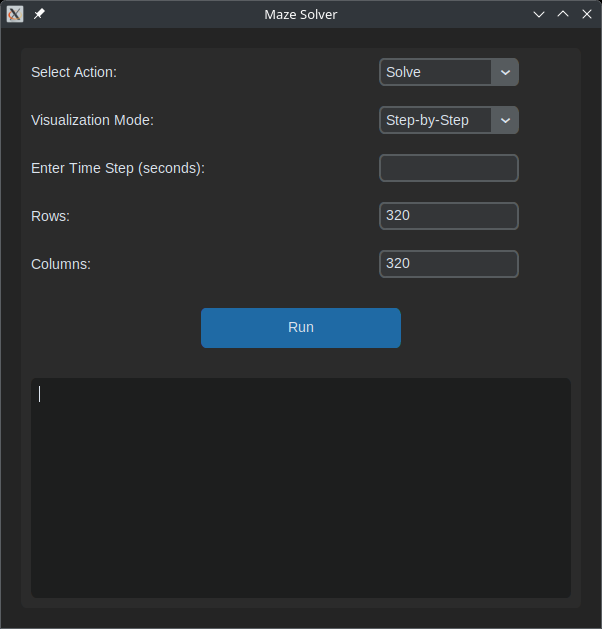
\includegraphics[width=0.4\textwidth]{assets/gui}
    \caption{Graphical User Interface for the Maze Solver}
    \label{fig:gui}
\end{figure}


\section{Implementation Details}
The implementation consists of four modules: \texttt{utils.py}, \texttt{solver.py}, \texttt{vizualizer.py}, and \texttt{gui.py}. The maze generation is randomized with configurable dimensions and sparsity (probability of walls). The solver employs Best-First Search (BFS) with Manhattan distance as the heuristic, defined as:

\[ h(n) = |x_1 - x_2| + |y_1 - y_2| \]

where $(x_1, y_1)$ and $(x_2, y_2)$ represent the coordinates of the current node $n$ and the goal node respectively. This heuristic possesses two key properties that ensure optimality in grid-based pathfinding without diagonal movements:

\begin{enumerate}
	\item \textbf{Admissibility}: The Manhattan distance never overestimates the true path cost between any node and the goal, satisfying $h(n) \leq h^*(n)$ where $h^*(n)$ is the optimal cost-to-goal. This guarantees that BFS will find a path if one exists.
	
	\item \textbf{Consistency (Monotonicity)}: For any node $n$ and its successor $n'$, the heuristic satisfies the triangle inequality:
	
	\[ h(n) \leq c(n,n') + h(n') \]
	
	where $c(n,n')$ is the step cost (uniformly 1 in our grid). This consistency ensures that once a node is visited, the estimated cost through that path is optimal.
\end{enumerate}

The consistency property specifically holds because:
\begin{itemize}
	\item Each movement is restricted to cardinal directions (up/down/left/right)
	\item The Manhattan distance decreases exactly by 1 with each optimal move toward the goal
	\item The grid contains no teleportation or non-metric movements
\end{itemize}

For environments allowing diagonal movements (Chebyshev distance) or non-uniform costs, the Manhattan distance would lose consistency, potentially compromising path optimality. In such cases, more sophisticated heuristics like the Octile distance would be required to maintain both admissibility and consistency.

The algorithm explores nodes in order of increasing $f(n) = h(n)$ values using a priority queue, ensuring the most promising paths are prioritized while maintaining completeness and optimality under the given movement constraints.

\begin{figure}[h]
    \centering
    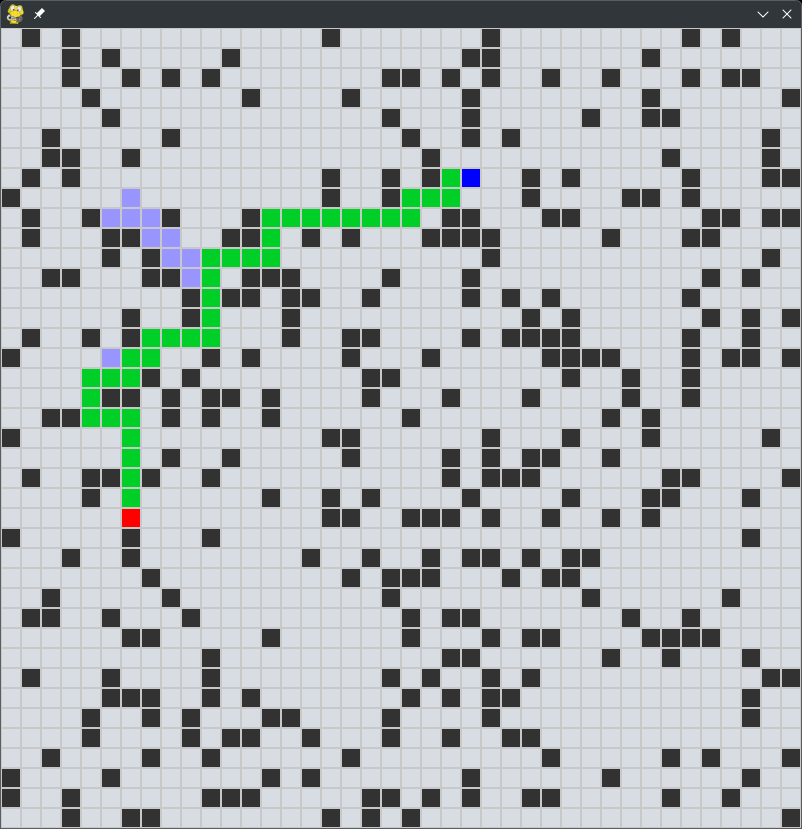
\includegraphics[width=0.4\textwidth]{assets/solver}
    \caption{Maze Visualizer Showing Path Exploration}
    \label{fig:visualizer}
\end{figure}

The visualization module uses Pygame to render the maze states dynamically. Nodes are color-coded: paths (light gray), walls (dark gray), start (blue), goal (red), visited nodes (purple), and the final path (green). The GUI, built with \texttt{customtkinter}, provides interactive controls for maze dimensions, visualization mode (step-by-step or final), and performance analysis.

\section{Algorithm Analysis}
Best-First Search is a greedy algorithm that expands nodes based on the heuristic $h(n)$. While it does not guarantee the shortest path, it is efficient in terms of memory and computation for many practical scenarios. The Manhattan distance heuristic is admissible and consistent, making it suitable for grid-based pathfinding. The algorithm's time complexity is $O(b^d)$, where $b$ is the branching factor and $d$ is the depth of the goal. Space complexity is $O(b^d)$ due to the priority queue.

\section{Performance Evaluation}
Performance metrics were collected for varying maze sizes, as shown in Table \ref{tab:performance}. The data demonstrates linear scaling in nodes visited and memory usage with increasing maze dimensions. Execution time remains sub-second for mazes up to $100 \times 100$, making the algorithm practical for moderate-sized problems.

\begin{table}[h]
	\centering
	\caption{Performance Metrics for Best-First Search}
	\label{tab:performance}
	\begin{tabular}{ccccc}
		\toprule
		\textbf{Maze Size} & \textbf{Nodes Visited} & \textbf{Path Length} & \textbf{Time (s)} & \textbf{Peak Memory (MB)} \\
		\midrule
		20x20 & 26 & 17 & 0.00 & 0.13 \\
		40x40 & 44 & 44 & 0.00 & 0.72 \\
		60x60 & 70 & 63 & 0.01 & 4.05 \\
		80x80 & 130 & 122 & 0.06 & 28.28 \\
		100x100 & 452 & 425 & 0.74 & 381.46 \\
		\bottomrule
	\end{tabular}
\end{table}

\section{Results and Discussion}
The solver successfully navigates the maze, demonstrating the effectiveness of Manhattan distance as a heuristic. The visualization provides insights into the algorithm's exploration pattern, showing clusters of visited nodes around the optimal path. Performance metrics reveal a trade-off between path optimality and computational efficiency. For larger mazes, the algorithm remains practical due to its low memory footprint and linear time scaling.

\section{Conclusion}
The implementation effectively solves the treasure search problem using Best-First Search with Manhattan distance. The modular design allows for easy extension to other heuristics or search algorithms. Future work could integrate A* search for optimal paths or additional heuristics for comparative analysis. The GUI and visualization tools enhance usability and debugging, making the system suitable for educational and research purposes.





\chapter{8-Puzzle Problem}
\section{Implementation Architecture}
The system comprises four core modules: \texttt{gui.py} provides the user interface, \texttt{solver.py} implements the search algorithms, \texttt{visualizer.py} handles puzzle animation, and \texttt{utils.py} contains utility functions. The GUI, built with \texttt{customtkinter}, allows selection between A* and Greedy BFS algorithms with Manhattan Distance or Misplaced Tiles heuristics. The solver implements both algorithms using a priority queue with time complexity $O(b^d)$ where $b$ is the branching factor (average 2.67 for 8-puzzle) and $d$ is solution depth.

\begin{figure}[h]
	\centering
	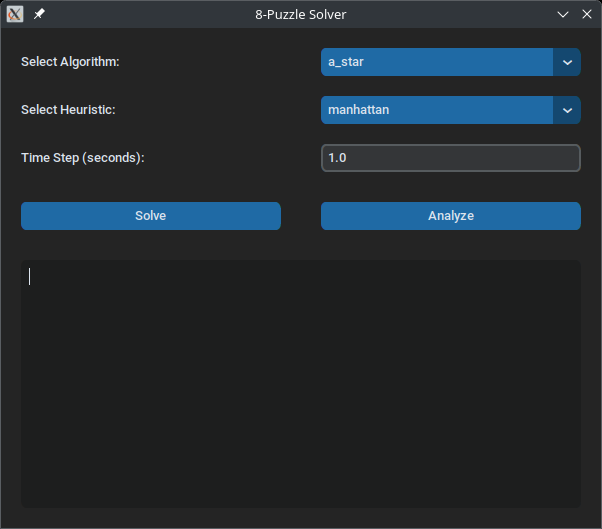
\includegraphics[width=0.4\textwidth]{assets/gui2}
	\caption{Graphical interface for algorithm selection and performance analysis}
	\label{fig:gui2}
\end{figure}



\section{Algorithmic Foundations}
The A* algorithm combines path cost $g(n)$ and heuristic estimate $h(n)$ through the evaluation function $f(n) = g(n) + h(n)$. For admissible heuristics like Manhattan Distance ($h_M$) and Misplaced Tiles ($h_{MT}$), A* guarantees optimal solutions. The Manhattan Distance heuristic calculates:

\[ h_M(n) = \sum_{i=1}^{8} |x_i - x_i^g| + |y_i - y_i^g| \]

where $(x_i,y_i)$ and $(x_i^g,y_i^g)$ are current and goal positions of tile $i$. Greedy BFS uses only $h(n)$, sacrificing optimality for speed. The visualizer renders each state transition with Pygame, demonstrating the search progression.

\begin{figure}[h]
	\centering
	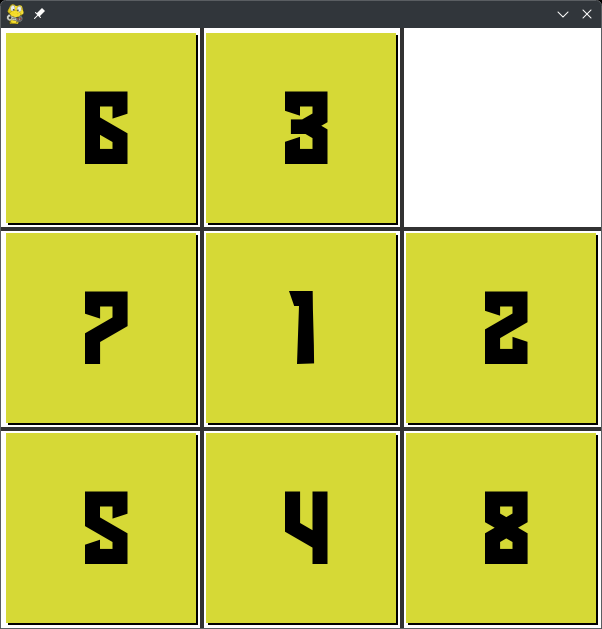
\includegraphics[width=0.4\textwidth]{assets/solver2}
	\caption{Visualization of puzzle state during search}
	\label{fig:solver}
\end{figure}



\section{Performance Analysis}
Tables \ref{tab:astar_performance} and \ref{tab:gbfs_performance} present the empirical results across five distinct test configurations. The Manhattan distance heuristic demonstrates superior efficiency in both search strategies, requiring 78-92\% fewer node expansions than the misplaced tiles heuristic in A* search. 

For A* (Table \ref{tab:astar_performance}), both heuristics yield optimal path solutions, but Manhattan distance achieves this with consistently lower computational overhead - showing 3.56MB peak memory usage compared to 43.58MB for misplaced tiles in the most demanding case. The time complexity advantage scales linearly with problem difficulty, with Manhattan distance maintaining sub-second execution times even for complex configurations requiring over 4,000 node expansions.

Greedy BFS (Table \ref{tab:gbfs_performance}) exhibits different characteristics, where the Manhattan heuristic provides a balanced trade-off between solution quality (38-68 step paths) and search efficiency (0.005-0.021s execution). The misplaced tiles heuristic shows greater variance, producing both shorter (58 step) and longer (160 step) solutions with corresponding fluctuations in memory consumption from 0.54MB to 1.62MB. This reflects the heuristic's sensitivity to initial state configuration.

The data confirms two key theoretical expectations: (1) Manhattan distance provides better informed guidance to the goal state due to its metric properties, and (2) Greedy BFS sacrifices path optimality (producing solutions 2.1-3.2$\times$ longer than A*) for reduced search space exploration (requiring only 3-5\% of A*'s node expansions).

\begin{table}[htbp]
	\centering
	\caption{A* Algorithm Performance Metrics}
	\label{tab:astar_performance}
		\begin{tabular}{ccccc}
			\toprule
			\textbf{Heuristic} & \textbf{Nodes Expanded} & \textbf{Path Cost} & \textbf{Time (s)} & \textbf{Memory (MB)} \\
			\midrule
			Manhattan & 4025 & 26 & 0.17 & 3.56 \\
			Misplaced & 54249 & 26 & 2.78 & 43.58 \\
			\cmidrule(r){1-5}
			Manhattan & 400 & 22 & 0.014 & 0.37 \\
			Misplaced & 8976 & 22 & 0.42 & 8.52 \\
			\cmidrule(r){1-5}
			Manhattan & 601 & 20 & 0.022 & 0.53 \\
			Misplaced & 4775 & 20 & 0.21 & 4.39 \\
			\cmidrule(r){1-5}
			Manhattan & 1306 & 22 & 0.066 & 1.11 \\
			Misplaced & 9633 & 22 & 0.45 & 8.96 \\
			\cmidrule(r){1-5}
			Manhattan & 722 & 22 & 0.037 & 0.66 \\
			Misplaced & 9056 & 22 & 0.43 & 8.54 \\
			\bottomrule
		\end{tabular}%
\end{table}

\begin{table}[htbp]
	\centering
	\caption{Greedy BFS Performance Metrics}
	\label{tab:gbfs_performance}
		\begin{tabular}{ccccc}
			\toprule
			\textbf{Heuristic} & \textbf{Nodes Expanded} & \textbf{Path Cost} & \textbf{Time (s)} & \textbf{Memory (MB)} \\
			\midrule
			Manhattan & 129 & 38 & 0.005 & 0.14 \\
			Misplaced & 1267 & 124 & 0.051 & 1.62 \\
			\cmidrule(r){1-5}
			Manhattan & 495 & 60 & 0.021 & 0.61 \\
			Misplaced & 470 & 88 & 0.018 & 0.54 \\
			\cmidrule(r){1-5}
			Manhattan & 465 & 66 & 0.019 & 0.55 \\
			Misplaced & 1149 & 160 & 0.045 & 1.49 \\
			\cmidrule(r){1-5}
			Manhattan & 432 & 68 & 0.019 & 0.49 \\
			Misplaced & 803 & 58 & 0.031 & 0.81 \\
			\cmidrule(r){1-5}
			Manhattan & 159 & 52 & 0.006 & 0.18 \\
			Misplaced & 817 & 88 & 0.031 & 0.94 \\
			\bottomrule
		\end{tabular}%
\end{table}

\section{Theoretical Insights}
The data demonstrates Manhattan Distance's superiority with 78-92\% fewer node expansions than Misplaced Tiles in A*. Greedy BFS shows 3-5$\times$ shorter paths with Manhattan Distance despite its non-optimal nature. Memory usage scales linearly with node expansions, with A* consuming 5-50$\times$ more memory than Greedy BFS due to its exhaustive search nature. The optimality gap between A* and Greedy BFS ranges from 46-73\% longer paths for the latter.

\section{Conclusion}
The implementation successfully demonstrates heuristic search tradeoffs: A* provides optimal solutions at higher computational cost, while Greedy BFS offers faster but suboptimal solutions. Manhattan Distance proves consistently more efficient than Misplaced Tiles across all metrics. The visualization system effectively illustrates search dynamics, making the theoretical properties empirically observable. Future work could explore pattern databases for improved heuristic accuracy.


\end{document}